\documentclass[]{article}
\usepackage[T1]{fontenc}
\usepackage{lmodern}
\usepackage{amssymb,amsmath}
\usepackage{ifxetex,ifluatex}
\usepackage{fixltx2e} % provides \textsubscript
% use upquote if available, for straight quotes in verbatim environments
\IfFileExists{upquote.sty}{\usepackage{upquote}}{}
\ifnum 0\ifxetex 1\fi\ifluatex 1\fi=0 % if pdftex
  \usepackage[utf8]{inputenc}
\else % if luatex or xelatex
  \ifxetex
    \usepackage{mathspec}
    \usepackage{xltxtra,xunicode}
  \else
    \usepackage{fontspec}
  \fi
  \defaultfontfeatures{Mapping=tex-text,Scale=MatchLowercase}
  \newcommand{\euro}{€}
\fi
% use microtype if available
\IfFileExists{microtype.sty}{\usepackage{microtype}}{}
\usepackage{longtable,booktabs}
\usepackage{graphicx}
% Redefine \includegraphics so that, unless explicit options are
% given, the image width will not exceed the width of the page.
% Images get their normal width if they fit onto the page, but
% are scaled down if they would overflow the margins.
\makeatletter
\def\ScaleIfNeeded{%
  \ifdim\Gin@nat@width>\linewidth
    \linewidth
  \else
    \Gin@nat@width
  \fi
}
\makeatother
\let\Oldincludegraphics\includegraphics
{%
 \catcode`\@=11\relax%
 \gdef\includegraphics{\@ifnextchar[{\Oldincludegraphics}{\Oldincludegraphics[width=\ScaleIfNeeded]}}%
}%
\ifxetex
  \usepackage[setpagesize=false, % page size defined by xetex
              unicode=false, % unicode breaks when used with xetex
              xetex]{hyperref}
\else
  \usepackage[unicode=true]{hyperref}
\fi
\hypersetup{breaklinks=true,
            bookmarks=true,
            pdfauthor={},
            pdftitle={},
            colorlinks=true,
            citecolor=blue,
            urlcolor=blue,
            linkcolor=magenta,
            pdfborder={0 0 0}}
\urlstyle{same}  % don't use monospace font for urls
\setlength{\parindent}{0pt}
\setlength{\parskip}{6pt plus 2pt minus 1pt}
\setlength{\emergencystretch}{3em}  % prevent overfull lines
\setcounter{secnumdepth}{0}

\author{}
\date{}

\begin{document}

\section{Introduction}\label{introduction}

This chapter will be about introduction to Elasticsearch-Logstash-Kibana
(ELK) stack and our underlying technologies. We will begin by explaining
some background on the ELK we use, ATLAS grid system and dCache billing
log files and more, then move on to how to get Docker running on your
system and finally how to get it set up to start working with. After
reading this introcuntion and the following chapters, we expect that you
will easily start running your own ELK instance on Docker.

\subsection{Distributed grid systems and dCache storage system used by
them}\label{distributed-grid-systems-and-dcache-storage-system-used-by-them}

In a ATLAS distributed grid site, its transfers and job efficiencies are
monitored by some central dashboard systems such as the Rucio and Big
PanDA. Each grid site has not been checked only by the latest status in
the dashboards, also by periodic checks such as nagios, availability
tests (e.g.~HammerCloud) and so on. Furthermore, many of these systems
are dealt with by many experts, central shifters and the national
computing facilities/groups with having several remote
meetings/communications they can work with. So, one grid site can
collaborate with different groups of people in different monitoring ways
simultaneously within the same experiment, in our case, ATLAS. This
allows us to distribute several types of monitoring and administration
tasks that are possible in both centralized systems and hierarchical
models {[}8{]}. As for a storage system of German ATLAS computing
Tier1/Tier2 sites, dCache storage system developed by DESY is widely
used. The dCache can use hierarchical storage management (e.g.~over many
RAID disks and tapes), provides mechanisms to automatically increase
performance and balance loads, increase resilience and availability
{[}9{]}. It also supplies advanced control systems and various grid
protocols to manage data as well as data workflow in each site.

\subsection{About Elasticsearch-Logstash-Kibana
(ELK)}\label{about-elasticsearch-logstash-kibana-elk}

What is the ELK stack, and why should we care? ELK stack deliver
actionable insights in real time for almost any type of structured and
unstructured data source, at any scale. From centralizing infrastructure
logs, traces, and metrics to deliver administrators. ELK is a combined
system that parse the records, collect and display information of
different log files or messages so that one can recall and display
specific records {[}4{]}. In our practical use-case, final outcomes
given by the Kibana dashbaord has been displayed by internal/external
dCache data workflow and information recorded by its billing log files
so far. Many organizations worldwide are using the ELK Stack for various
mission-critical use cases in ATLAS and some large Tier1s as well.

\subsection{Docker}\label{docker}

Docker has become the de facto standard that developers and system
administrators use for packaging, deploying, and running distributed
applications. It provides tools for simplifying mission-critial
operations and administrations by enabling developers to create
templates called images that can be used to create lightweight virtual
machines called containers, which include their applications and all of
their applications' dependencies. These lightweight virtual machines can
be promoted through testing and production environments where system
administrators deploy and run them.

\begin{figure}[htbp]
\centering
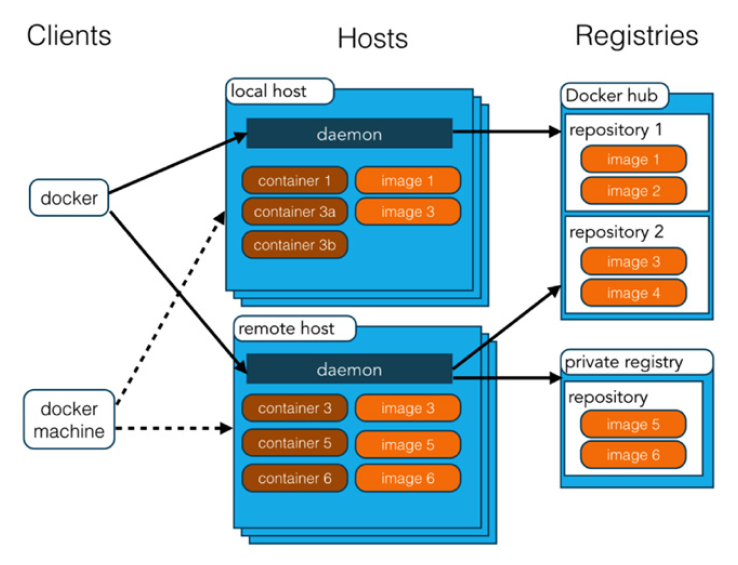
\includegraphics{images/docker.png}
\caption{How docker works.}
\end{figure}

Similar to the popular version control software Git, Docker has a social
aspect, in that developers and administrators are able to share their
images via Docker Hub (Figure 1-1). Docker is an open-source solution
that runs natively on Linux but also works on Windows and Mac using a
lightweight Linux distribution and VirtualBox. Many tools have also
grown up around Docker to make it easier to manage and orchestrate
complex distributed applications such as grid monitoring tools and the
ELK stack.

\subsection{Docker compose and Gantry
command}\label{docker-compose-and-gantry-command}

Docker compose is a tool for defining and running multi-container Docker
applications. With docker-compose command, one uses a YAML file to
configure the application's services. Then, with a single docker-compose
command, the one create and start all the services from its
configuration.

The docker-compose command works in all environments we need:
production, staging, development, testing, as well as Continuous
Integration (CI) workflows. We can learn more about each case in our
cookbook chapter. In our settings, we simply implemented a wrapper
command, called mad-gantry, which is a wrapper of docker-compose, making
easier to generate docker template and docker instance template for
different monitoring tools we have developed such HappyFace and now the
ELK stack.

The concept of our `Gantry' is following

\begin{itemize}
\itemsep1pt\parskip0pt\parsep0pt
\item
  Simple design (pre-defined YAML files and its settings are given, and
  easily re-generated)
\item
  A wrapper of docker-compose
\item
  Easily distributed or separated by one config file
\item
  Standardisable and adaptable for many sites, monitoring tools and
  different local settings
\item
  Checking if services are running
\item
  Syncronising the tools and configurations with the code in the Git
  repository
\end{itemize}

\section{Settings}\label{settings}

Our settings running with test data of GoeGrid Tier2 site are

\begin{itemize}
\itemsep1pt\parskip0pt\parsep0pt
\item
  CPU: Intel(R) Xeon(R) CPU E5-2630 v4 @ 2.20GHz x 40 Cores
\item
  Memory: 65 GB
\item
  HDD and SSD: 1 TB
\item
  Operating system: Scientific Linux 7.5
\item
  Docker: 1.12.6
\item
  Docker Compose: 1.9.0
\item
  Size of dCache billing log (10 years): 442 GB
\end{itemize}

\begin{longtable}[c]{@{}cccc@{}}
\toprule\addlinespace
Size of billing (GB) & Years & Index size & Elapsed time (hours)
\\\addlinespace
\midrule\endhead
72 & 1 & 156.2 & 13.5
\\\addlinespace
129 & 2 & 296.8 & 27.3
\\\addlinespace
365 & 4 & 512.6 & 131.9
\\\addlinespace
430 & 8 & X & Y
\\\addlinespace
442 & 10 & X & Y
\\\addlinespace
\bottomrule
\end{longtable}

\section{Logstash}\label{logstash}

Logstash is a tool to collect, process, and forward events and log
messages. Collection is accomplished via configurable input plugins
including raw socket/packet communication, file tailing, and several
message bus clients. There are many built-in patterns and plugins that
are supported out-of-the-box by Logstash for filtering items such as
words, numbers, and dates. If we cannot find the pattern we need, we can
write own custom pattern. In our dCache billing log use-case so far, we
put our pattern based on a standard dCache logstash template
{[}4{]}{[}5{]}.

\subsection{Logstash configuraiton for dCache billing
log}\label{logstash-configuraiton-for-dcache-billing-log}

The pattern and pipeline files are defined by
`customs/*/logstash/pattern' and `customs/*/logstash/pipeline'.

\begin{itemize}
\itemsep1pt\parskip0pt\parsep0pt
\item
  Some examples of dCache log pattern
\end{itemize}

The raw information about all dCache activities can be found in
/var/lib/dcache/billing/YYYY/MM/billing-YYYY.MM.DD. A typical line looks
like

\begin{verbatim}
 05.31 22:35:16 [pool:pool-name:transfer] [000100000000000000001320,24675] \
 myStore:STRING@osm 24675 474 true {GFtp-1.0 client-host-fqn 37592} {0:""}
\end{verbatim}

The first bracket contains the pool name, the second the pnfs ID and the
size of the file which is transferred. Then follows the storage class,
the actual amount of bytes transferred, and the number of milliseconds
the transfer took. The next entry is true if the transfer was a wrote
data to the pool. The first braces contain the protocol, client FQN, and
the client host data transfer listen port. The final bracket contains
the return status and a possible error message. The billing info keeps
such general accountings about the cell, pool, door and actions, such as
removal, move and so on, for listing the details of their requests. The
output of those requests often contains useful information for
describing details of the transfers and solving problems. For instance,
the following patterns describe a general (classical) transfer request
and a store request. Each accounting line should have appropriate fields
such as datetime, PNFS ID, file size, transfered time, protocol, pool or
door names, error and so on. The fields are already defined by
`customs/*/logstash/pattern' and its pattern file is called by
`customs/*/logstash/pipeline'.

\begin{verbatim}
 TRANSFER_CLASSIC %{BILLING_TIME:billing_time} %{CELL_AND_TYPE} %{PNFSID_SIZE} %{PATH} \
 %{SUNIT} %{TRANSFER_SIZE} %{TRANSFER_TIME} %{IS_WRITE} %{PROTOCOL} %{DOOR} %{ERROR}

 STORE_CLASSIC %{BILLING_TIME:billing_time} %{CELL_AND_TYPE} %{PNFSID_TSIZE} %{PATH} \
 %{SUNIT} %{TRANSFER_TIME} %{QUEUE_TIME} %{ERROR}
\end{verbatim}

\section{Elasticsearch}\label{elasticsearch}

Elasticsearch is a real-time distributed search and analytics engine
{[}4{]}{[}6{]}. It allows one to explore data at a speed and at a scale
never before possible. It is used for full-text search, structured
search, analytics, and all in combination. Elasticsearch is an
open-source search engine built on top of Apache Lucene, a fulltext
search-engine library. However, Elasticsearch is much more than just
Lucene and much more than just full-text search. It can also be
described as follows:

\begin{itemize}
\itemsep1pt\parskip0pt\parsep0pt
\item
  A distributed real-time document store where every field is indexed
  and searchable
\item
  A distributed search engine with real-time analytics
\item
  Capable of scaling to hundreds of servers and petabytes of structured
  and unstructured data
\end{itemize}

And it packages up all this functionality into a standalone server that
applications can talk to via a simple RESTful API, using a web client
from our favorite programming language, or even from the command line.

For instance, after starting our service up, our simplest example is
directly sending a query to the Elasticsearch instance (port 9200 in
this case) and get number of indices stored.

\begin{verbatim}
  $ curl 'localhost:9200/_cat/indices?v'

  health status index                  uuid                   pri rep docs.count
  yellow open   dcache-billing-2017.10 9ocm5mfoQX255Z8Z4NWwrA   5   1   33336024
  yellow open   dcache-billing-2017.09 bz1ZBIa4SmqetFGBpqruWA   5   1   17306766
  yellow open   dcache-billing-2018.02 iFuFB03PR_SsNNpf6sXpxw   5   1   25118420
  yellow open   dcache-billing-2018.01 HitUUihaRuGBnd47Ma98Bg   5   1   24001272
  yellow open   dcache-billing-2017.05 rnU_rxhcTt6Y-D6AeWxy8A   5   1   23641828
  yellow open   dcache-billing-2017.11 8s3hp4lBRzatjMzXDaNbUQ   5   1   49539540
  yellow open   dcache-billing-2018.04 vRUN0b08T4iZrvyNpxOcgA   5   1   26639090
  yellow open   dcache-billing-2018.12 GFhoMTqfSWKO80lp6iurfg   5   1   63447534
  yellow open   dcache-billing-2017.07 cleYoAc-QM2DgcpfiJnj6Q   5   1   31308502
  yellow open   dcache-billing-2018.11 QJxVUAqESSOGumiG5lk1cA   5   1   48383944
  yellow open   dcache-billing-2018.07 gfCszQ_4RUulIjn42guNUw   5   1   16616834
  green  open   .kibana                E-J_GSkdRj22BN7DQHMN_Q   1   0         27
  yellow open   dcache-billing-2019.04 A9Ic3--tQjaML_Zg_daFXA   5   1   11335536
  yellow open   dcache-billing-2018.09 MkD363YHRUqsIAZvTMCsCA   5   1   29330778
\end{verbatim}

\section{Kibana}\label{kibana}

\begin{figure}[htbp]
\centering
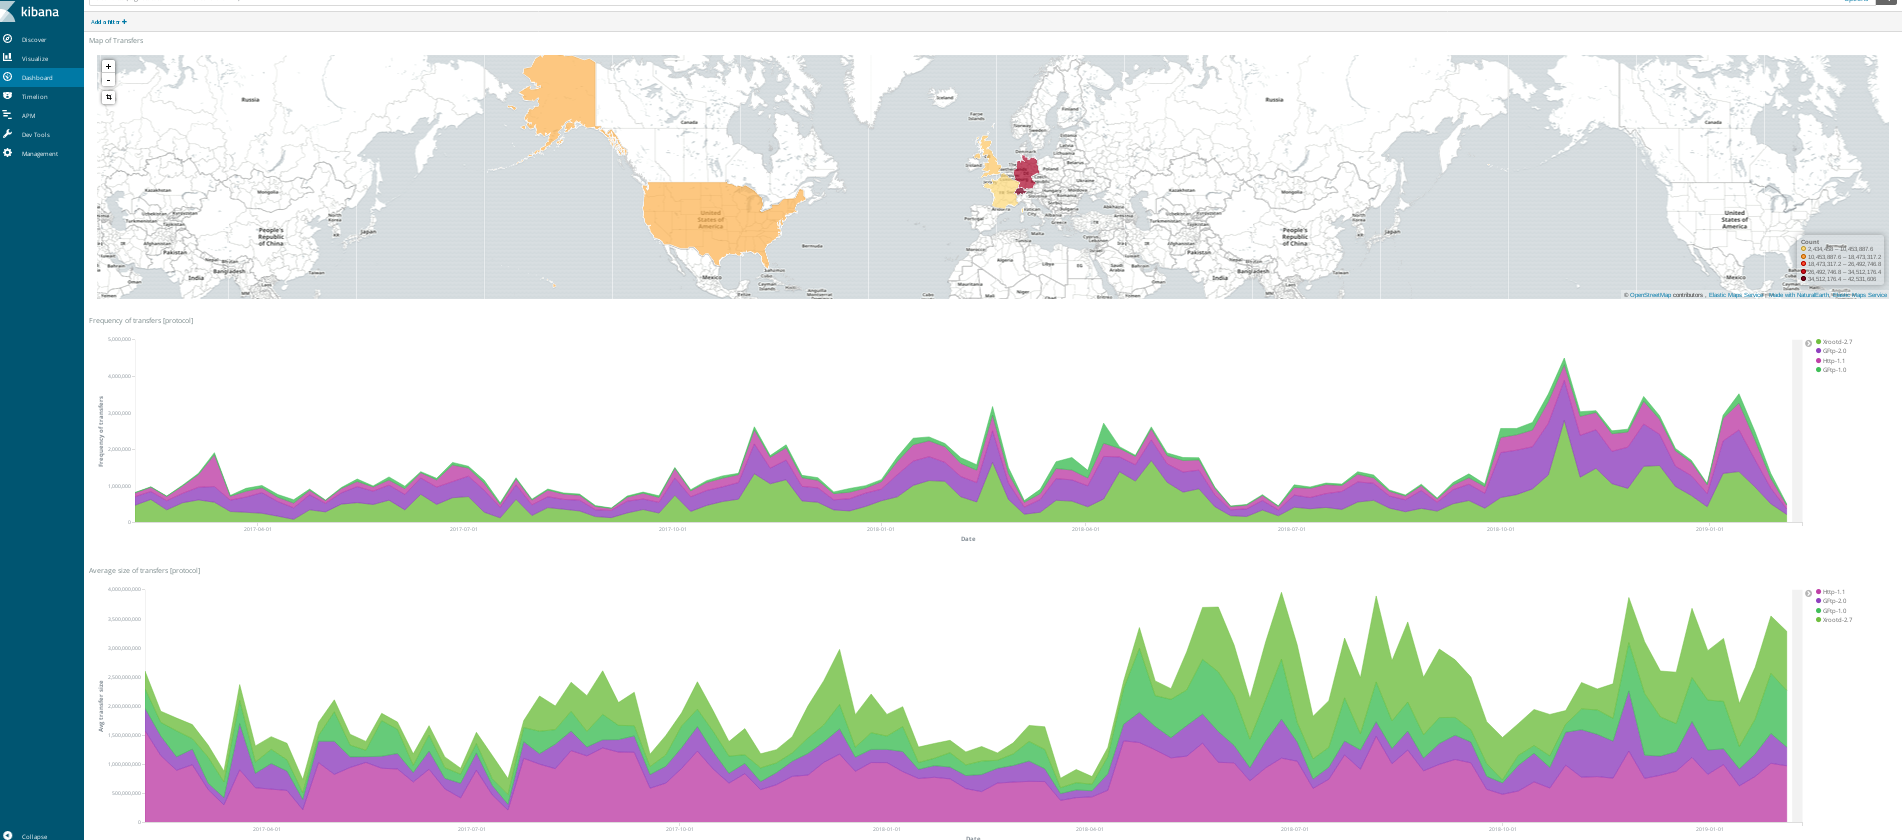
\includegraphics{images/kibana.png}
\caption{Main Dashboard}
\end{figure}

Kibana is an open source analytics and visualization platform designed
to work with Elasticsearch {[}4{]}{[}6{]}. We use Kibana to search,
view, and interact with data stored in Elasticsearch indices. We can
easily perform the data analysis and visualize our data in a variety of
charts, tables, and maps. Kibana makes a large local site easy to
understand large volumes of data, for instance, dCache billing log. Its
simple, browser-based interface enables you to quickly create and share
dynamic dashboards that display changes to Elasticsearch queries in real
time.

\begin{figure}[htbp]
\centering
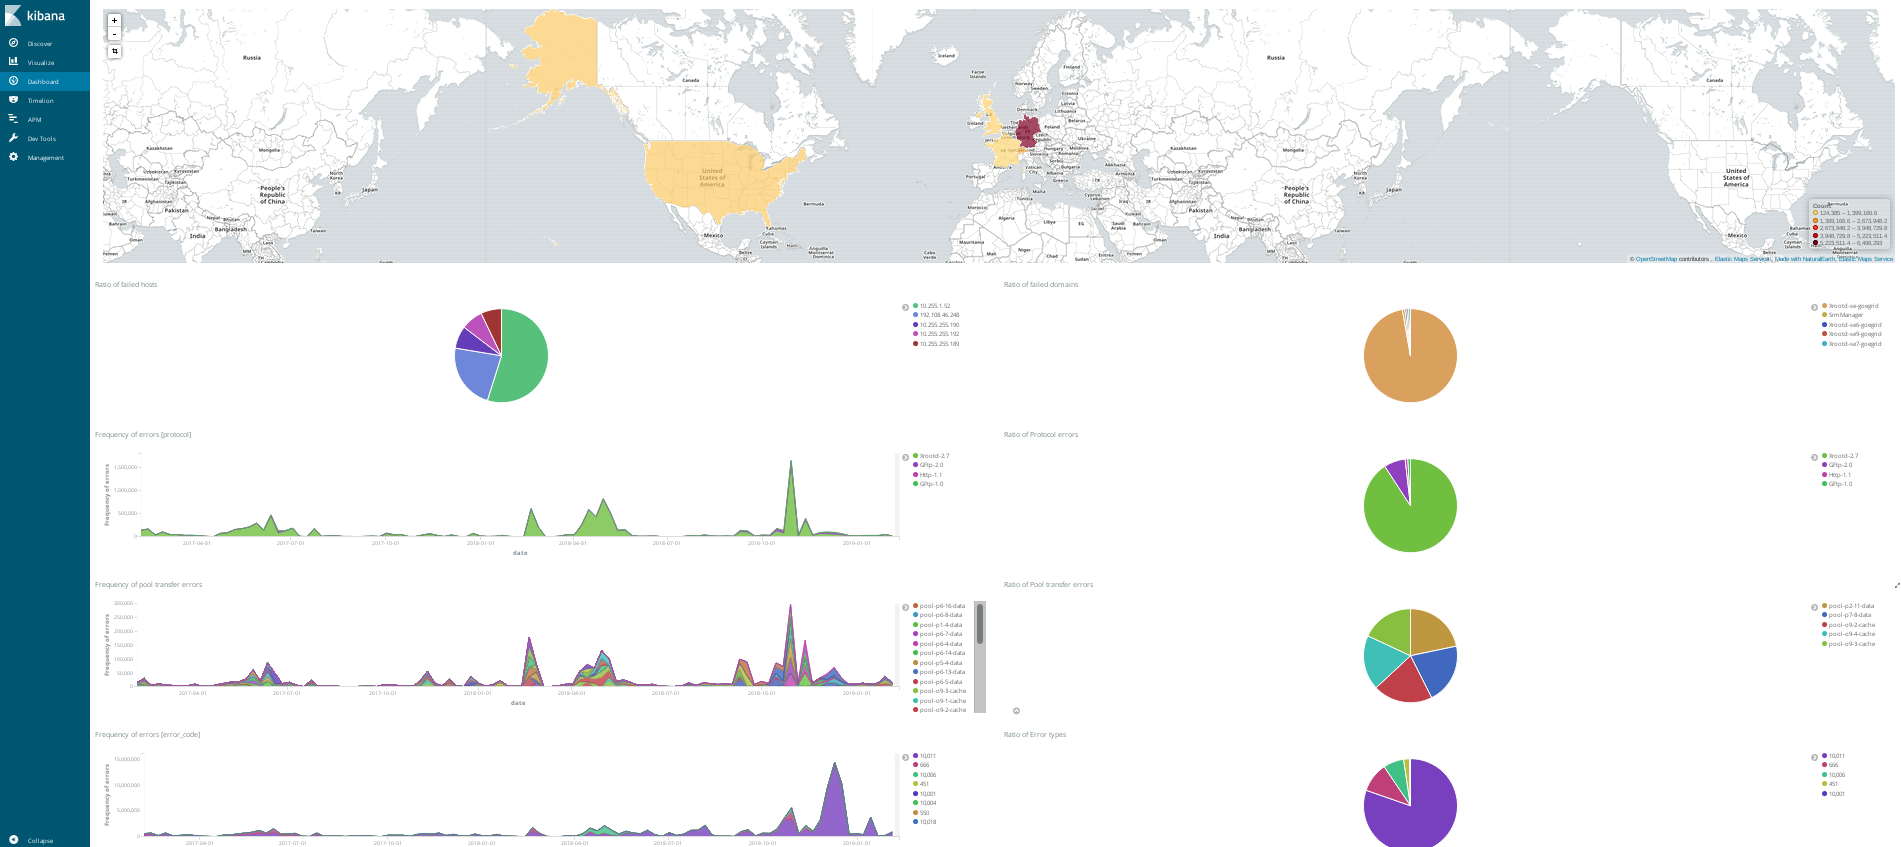
\includegraphics{images/kibana_error.png}
\caption{Main Error Dashboard}
\end{figure}

\section{Cookbook}\label{cookbook}

\subsection{Running ELK stack in a ATLAS Tier2
site}\label{running-elk-stack-in-a-atlas-tier2-site}

\begin{itemize}
\item
  Cloning the main command and generating ELK templates

  \$ git clone https://github.com/HappyFaceGoettingen/mad-gantry.git

  \$ cd mad-gantry

  \$ ./mad-gantry -b -t templates/docker-elk

  \$ ./mad-gantry -D -a setup

  \$ ls payloads/data/GoeGridELK

  billing elasticsearch\_index\_data
\item
  Copy billing logs into the billing directory (Note: indices will be
  kept in the `elasticsearch\_index\_data' directory)
\item
  Turn GoeGridELK instance up

  \$ ./mad-gantry -s GoeGridELK -a up

  \$ docker ps
\end{itemize}

\subsection{Configuration files and
templates}\label{configuration-files-and-templates}

There are some templates for ELK and dCache. These can most easily be
configured by copying them. Please note the templates of ELK used for
the test instance above mentioned can be found in
`configs/customs/GoeGridELK' and the templates are copied into
`ship/GoeGridELK' directory when it is set up. The interal configuration
parameters in the template files, such as `\textbf{SITE}',
`\textbf{PORT}' and so, on are adjusted by a configuration of
`ticket.conf'.

For instance, the site names and the docker images of `GoeGridELK' are
defined by Tier3 section of the `ticket.conf' file.

\begin{verbatim}
  ## ALL level3 sites (= Level3), level 3 sites are not in a tree structure
  ALL_LEVEL3_SITES=(AdminServer ApplicationBuilder GoeGridELK)
  ALL_LEVEL3_IMAGES=("happyface/admin-server.el7" "" "happyface/kibana")
  ALL_LEVEL3_HOSTS=($CLOUD0 $CLOUD0 $CLOUD0)
  ALL_LEVEL3_PORTS=(101 102 103)
  ALL_LEVEL3_SHIPS=("" "" "docker-elk")
\end{verbatim}

When the GoeGridELK and setup option of the gantry command are called,
the ship YAML file (ship/GoeGridELK/docker-compose.yml) generated and
the custom tempalates are copied (from `configs/customs/GoeGridELK') to
`payloads/sites/GoeGridELK'.

\begin{itemize}
\itemsep1pt\parskip0pt\parsep0pt
\item
  configs/customs/GoeGridELK/kibana/kibana.yml
\end{itemize}

Default Kibana configuration from kibana-docker.

\begin{verbatim}
  ## from https://github.com/elastic/kibana-docker/blob/master/build/kibana/config/kibana.yml
  #
  server.name: kibana
  server.host: "0"
  elasticsearch.url: http://__SITE__elasticsearch:__PORT__
  
  ## Disable X-Pack
  ## see https://www.elastic.co/guide/en/x-pack/current/xpack-settings.html
  ##     https://www.elastic.co/guide/en/x-pack/current/installing-xpack.html#xpack-enabling
  #
  xpack.security.enabled: false
  xpack.monitoring.enabled: false
  xpack.ml.enabled: false
  xpack.graph.enabled: true
  xpack.reporting.enabled: false
  xpack.grokdebugger.enabled: false
\end{verbatim}

\begin{itemize}
\itemsep1pt\parskip0pt\parsep0pt
\item
  ship/GoeGridELK/docker-compose.yml
\end{itemize}

A final template for Docker Compose

\begin{verbatim}
 Version: "2.0"
    services:
    
    # ELK framework Ship Platform
    goegridelkelasticsearch:
    image: happyface/elasticsearch
    volumes:
       - "/home/gen/mad-gantry/payloads/ssh:/root/.ssh"
       - "/home/gen/mad-gantry/payloads/data/GoeGridELK/billing:/billing"
       - "/home/gen/mad-gantry/payloads/sites/GoeGridELK/elasticsearch/elasticsearch.yml:/usr/share/elasticsearch/config/elasticsearch.yml"
       - "/home/gen/mad-gantry/payloads/data/GoeGridELK/elasticsearch_index_data:/usr/share/elasticsearch/data"
    ports:
       - "9200:9200"
       - "9300:9300"
    environment:
      ES_JAVA_OPTS: "-Xmx7g -Xms7g"
    networks:
       - elk
    .......
\end{verbatim}

\subsection{Manipulating Kibana
Visualisation}\label{manipulating-kibana-visualisation}

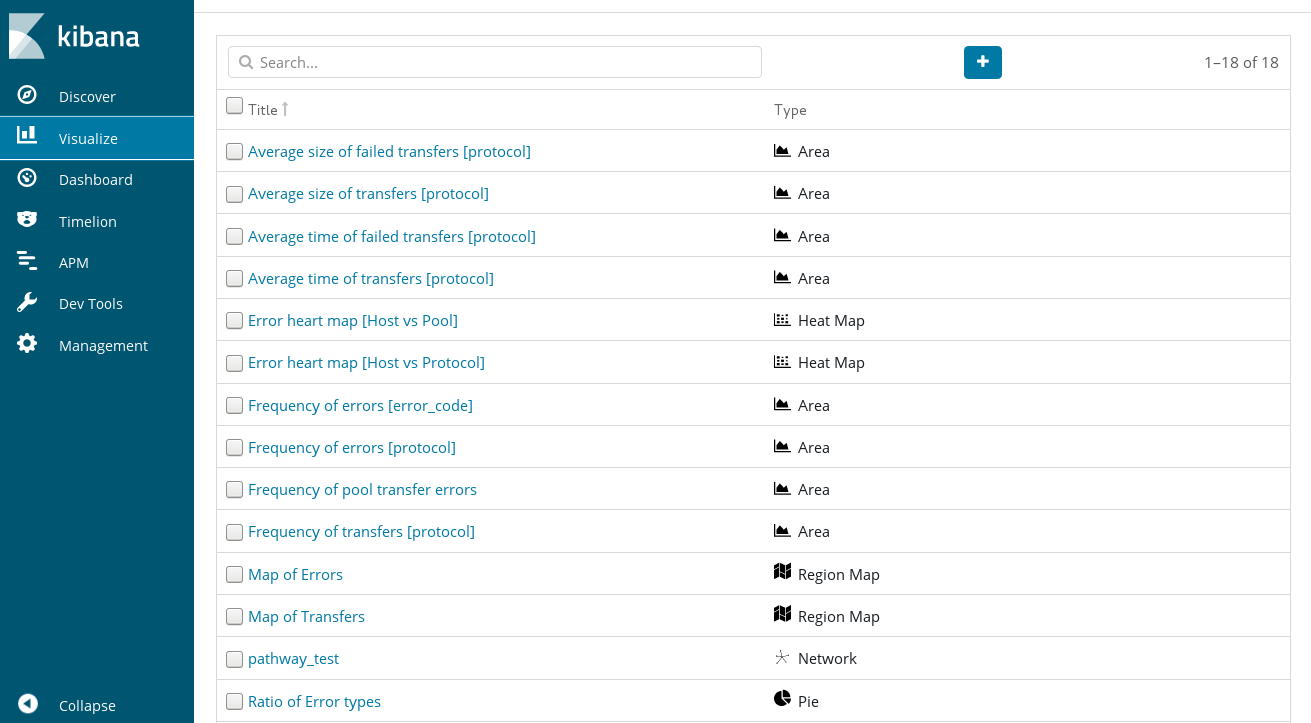
\includegraphics{images/kibana_vis1.png}
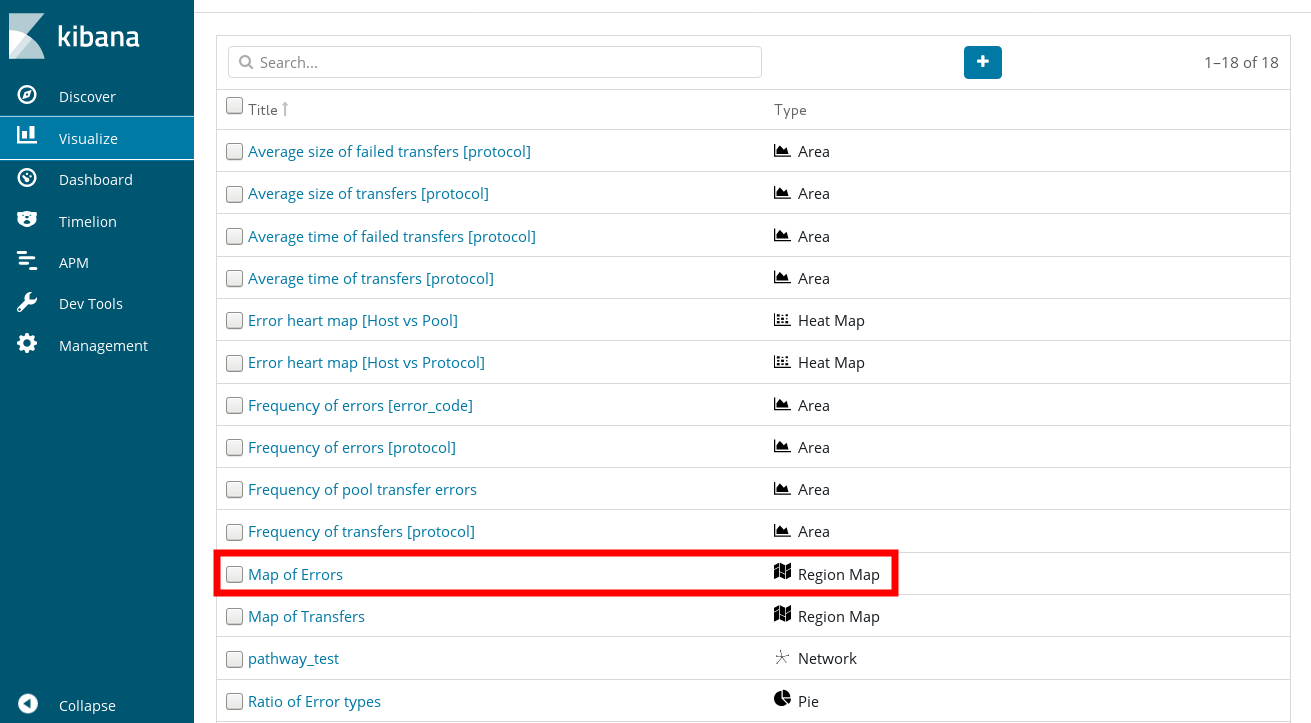
\includegraphics{images/kibana_vis2.png} The Kibana web interface
contains under the menu point ``Visualize'' tab listing from all plots
we created. The visualisation plots can also be redirected.

\subsection{Manipulating Kibana
Dashboard}\label{manipulating-kibana-dashboard}

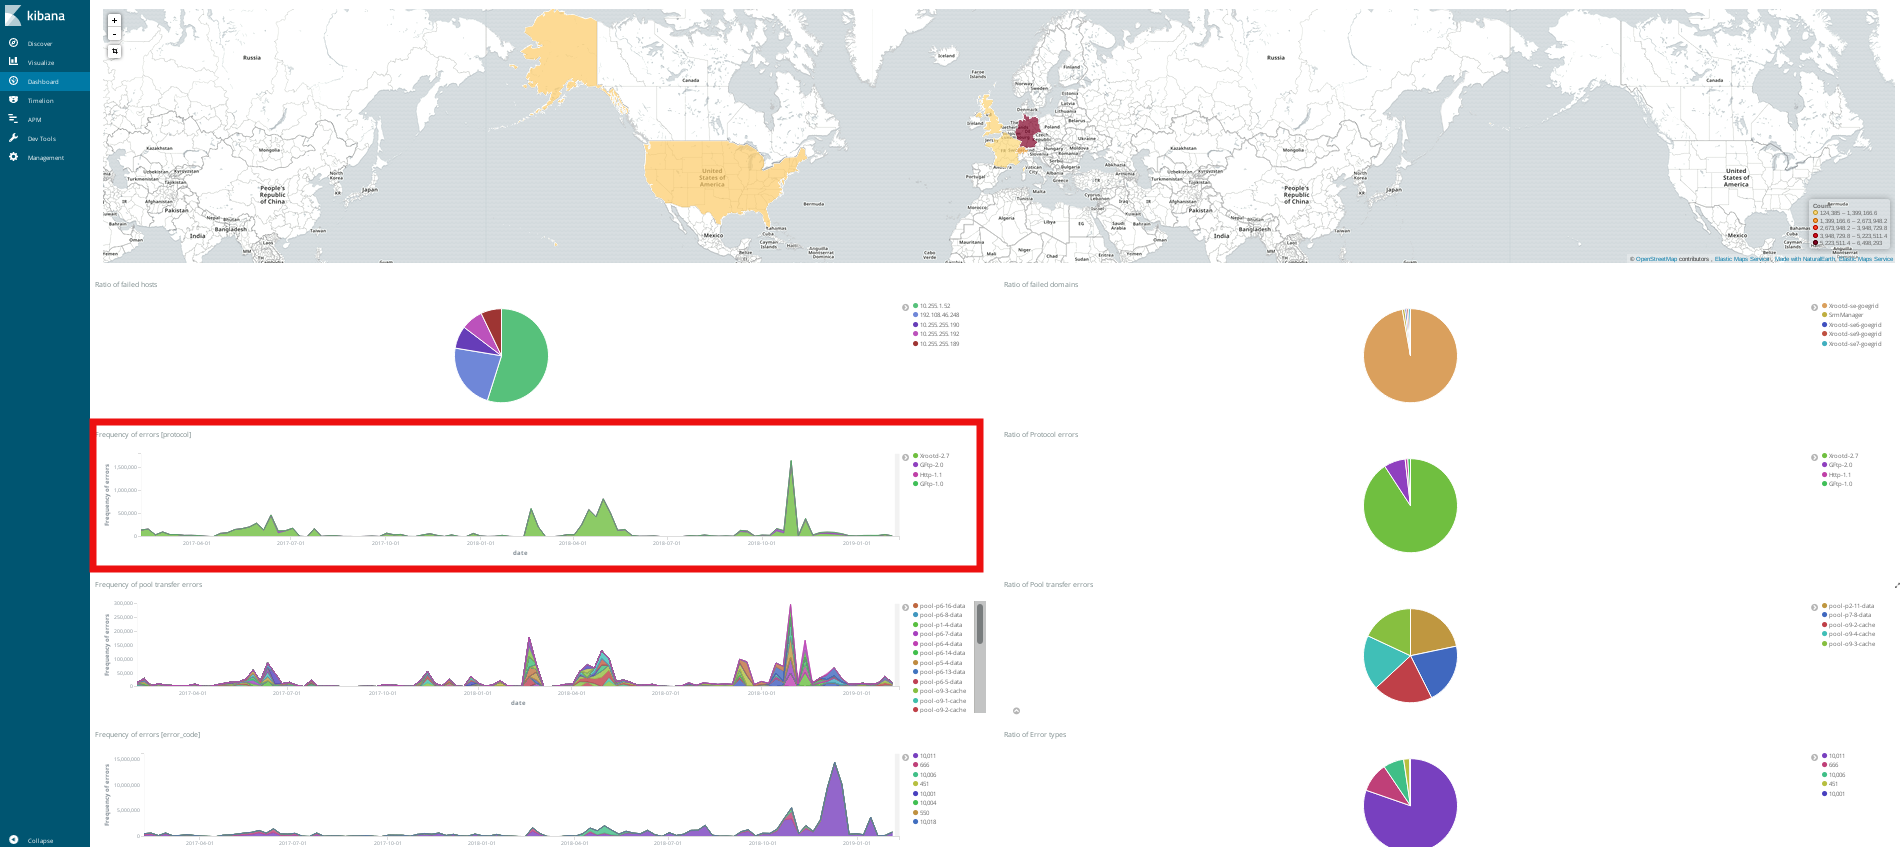
\includegraphics{images/kibana_main1.png} Each visualisation plot is
gathered and sorted by the main dashboard, so that one changes the
visualisation plot it will affect the dashboard view.

\subsection{Saving Kibana dashboard}\label{saving-kibana-dashboard}

In our case, we implemented our own darshboard (ID:
WeXmuoICywmhE8FvCht). So, exporting the JSON output, and re-using it
when the service is up again.

\begin{verbatim}
 $ id=WeXmuoICywmhE8FvCht
 $ export_url="http://localhost:20261/api/kibana/dashboards/export?dashboard=$id"
 $ GET "$export_url" > export.json

 $ import_url="http://localhost:20261/api/kibana/dashboards/import"
 $ curl -u elastic:changeme -k -XPOST "$import_url" \
     -H 'Content-Type: application/json' -H "kbn-xsrf: true" -d @export.json
\end{verbatim}

\subsection{Command snippets for
Elasticsearch}\label{command-snippets-for-elasticsearch}

There are many client tools for Elasticsearch. These can most easily be
communicated through RESTful web service in Elasticsearch engine.

\begin{itemize}
\item
  List indexes

  \$ curl 'localhost:9200/\_cat/indices?v'
\item
  Filter if error\_code in billing log is `0'

  \$ curl -XPOST 'localhost:9200/\_search' -d `\{``query'': \{ ``bool'':
  \{ ``filter'': \{ ``term'': \{``error\_code'': ``0''\} \} \} \} \}'
\item
  Simple matches using pool\_name in `billing log'

  \$ curl -XPOST 'localhost:9200/\_search?pretty=true' -d `\{``query'':
  \{ ``match\_all'': \{\} \} \}'

  \$ curl -XPOST 'localhost:9200/\_search?pretty=true' -d `\{``query'':
  \{ ``match'': \{ ``pool\_name'': ``pool-p1-1-data'' \} \} \}'
\item
  Aggregations

  \$ curl -XPOST `localhost:9200/\emph{search' -d '\{``aggs'': \{
  ``all\_interests'': \{ ``terms'': \{``field'': ``size''\} \} \} \}' \$
  curl -XPOST 'localhost:9200/}search' -d `\{``aggs'': \{ ``queries'':
  \{ ``terms'': \{``field'': ``size''\} \} \} \}'

  \$ curl -XPOST `localhost:9200/\emph{search' -d '\{``query'': \{
  ``match'': \{ ``pool\_name'': ``pool-p1-1-data'' \} \}, ``aggs'': \{
  ``all\_interests'': \{ ``terms'': \{``field'': ``size''\} \} \} \}' \$
  curl -XPOST 'localhost:9200/}search' -d `\{``query'': \{ ``match'': \{
  ``pool\_name'': ``pool-p1-1-data'' \} \}, ``aggs'': \{ ``queries'': \{
  ``terms'': \{``field'': ``size''\} \} \} \}'
\end{itemize}

\section{Reference}\label{reference}

{[}1{]} Docker, https://www.docker.com/

{[}2{]} Docker Hub, https://hub.docker.com/

{[}3{]} Docker Compose, https://docs.docker.com/compose/

{[}4{]} ELK Stack, https://www.elastic.co/elk-stack

{[}5{]} Logstash, https://www.elastic.co/products/logstash

{[}6{]} Elasticsearch, https://www.elastic.co/products/elasticsearch

{[}7{]} Kibana, https://www.elastic.co/products/kibana

{[}8{]} Campana, S., \& Atlas Collaboration. (2014). Evolution of the
ATLAS distributed computing system during the LHC long shutdown. In
Journal of Physics: Conference Series (Vol. 513, No. 3, p.~032016). IOP
Publishing.

{[}9{]} dCache, https://www.dcache.org/

\end{document}
